{Examples and Definitions}

\textbf{Problem to prove:} Construct both a know-show table and a first attempt at a formal proof of the following proposition.

\begin{prop}
    Let \( a, b \in \N \). If \( a^2 = b^3 \) and \( a \) is even, then \( 4 \mid a \).
\end{prop}

\subsection{Exploratory Work/Examples}

\textbf{Strategy:} 
To find four pairs of natural numbers \( (a, b) \) such that \( a^2 = b^3 \) and \( a \) is even, I modified my approach:
\begin{itemize}
    \item Filtered \( a \) to include only even numbers.
    \item Verified whether \( \sqrt[3]{a^2} \) is an integer and that \( b^3 = a^2 \).
    \item Added additional columns to check if \( a \) is even and ensure that both \( a \) and \( b \) satisfy the conditions for being natural numbers.
\end{itemize}

\textbf{Excel Formulas Used:}
\begin{itemize}
    \item Column A: Even natural numbers \( a \).
        \begin{itemize}
            \item Formula: \texttt{=even a value}
        \end{itemize}
    \item Column B: Squares of \( a \) (\( a^2 \)).
        \begin{itemize}
            \item Formula: \texttt{=POWER(A2, 2)}
        \end{itemize}
    \item Column C: Cube root of \( a^2 \) (\( \sqrt[3]{a^2} \)).
        \begin{itemize}
            \item Formula: \texttt{=POWER(B2, 1/3)}
        \end{itemize}
    \item Column D: Verification column for \( b^3 \) (\( b^3 \in \N \)).
        \begin{itemize}
            \item Formula: \texttt{=IF(AND(C2>0, C2=INT(C2)), C2*C2*C2 \& "$\in\mathbb{N}$", "b$\notin\mathbb{N}$")}
        \end{itemize}
    \item Column E: Even or Odd verification for \( a \).
        \begin{itemize}
            \item Formula: \texttt{=IF(A2=INT(A2), IF(MOD(A2,2)=0, "Even", "Odd"), "Not an Integer")}
        \end{itemize}
    \item Column F: Final check for Even and Natural.
        \begin{itemize}
            \item Formula: \texttt{=IF(AND(A2>0, A2=INT(A2), MOD(A2,2)=0, C2>0, C2=INT(C2)), "Natural and Even", "False")}
        \end{itemize}
\end{itemize}

\textbf{Results:} The four pairs satisfying \( a^2 = b^3 \), with \( a \) even, are:
\begin{center}
    \begin{tabular}{|c|c|c|c|}
    \hline
    \( a \) & \( a^2 \) & \( b \) & \( b^3 \) \\
    \hline
    8 & 64 & 4 & 64 \\
    64 & 4096 & 16 & 4096 \\
    216 & 46656 & 36 & 46656 \\
    512 & 262144 & 64 & 262144 \\
    \hline
    \end{tabular}
\end{center}

\textbf{Spreadsheet Screenshot:}
\begin{center}
    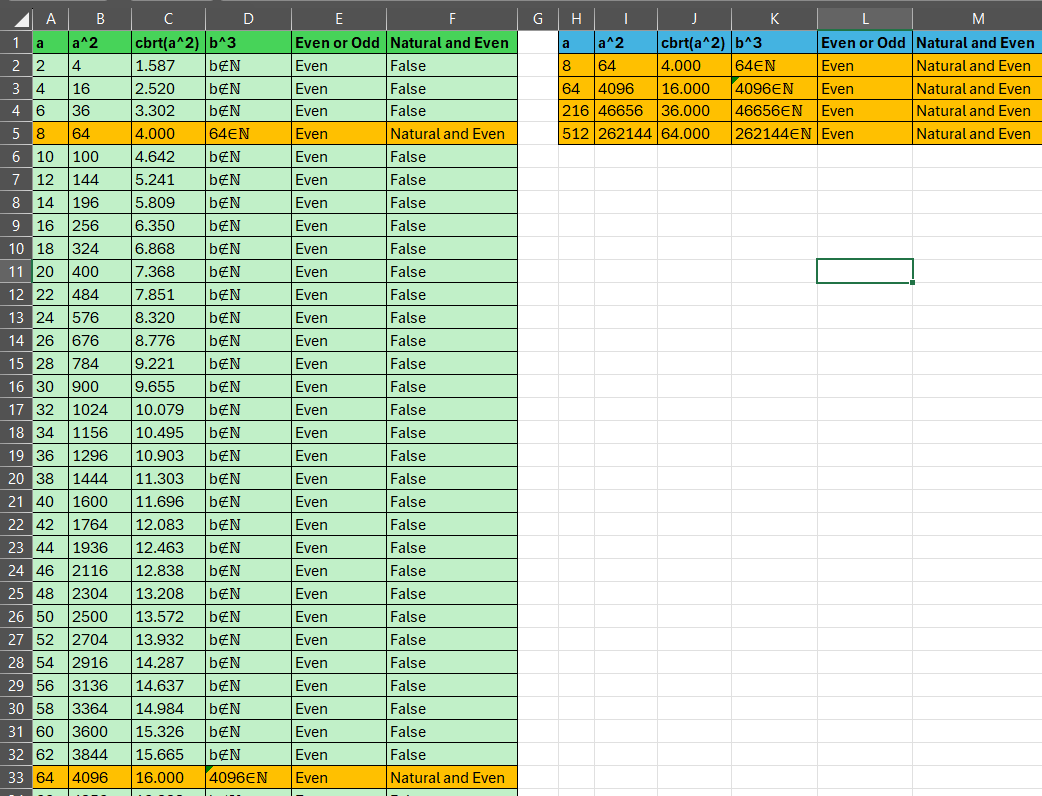
\includegraphics[width=\textwidth]{s.png}

\end{center}

\newpage

\subsection{Know-Show Table (\( a^2 = b^3 \) and \( a \) even \( \implies 4 \mid a \))}

\begin{center}
    \begin{tabular}{|p{.1\textwidth}|p{.6\textwidth}|p{.2\textwidth}|}
    \hline
    \textbf{Step} & \textbf{Know} & \textbf{Reason} \\
    \hline
        P1 & \( a^2 = b^3 \) & Hypothesis \\
    \hline
        P2 & \( a \) is even (\( a = 2k \)) & Hypothesis \\
    \hline
        P3 & \( (2k)^2 = b^3 \) & Substitution \\
    \hline
        P4 & \( 4k^2 = b^3 \) & Algebra \\
    \hline
        P5 & \( b \) is even (\( b = 2m \)) & Cubes divisible by 4 imply base divisible by 2 \\
    \hline
        P6 & Substituting \( b = 2m \): \( 4k^2 = (2m)^3 \) & Substitution \\
    \hline
        P7 & \( 4k^2 = 8m^3 \) & Algebra \\
    \hline
        P8 & \( k^2 = 2m^3 \) & Divide by 4 \\
    \hline
        P9 & \( k \) is even (\( k = 2n \)) & Squares divisible by 2 imply base divisible by 2 \\
    \hline
        Q1 & \( a = 4n \) & Substituting \( k = 2n \) into \( a = 2k \) \\
    \hline
    \textbf{Step} & \textbf{Show} & \textbf{Reason} \\
    \hline
    \end{tabular}
\end{center}

\newpage

\subsection{First Draft of Proof}

\begin{proof}
    Assume \( a^2 = b^3 \), and \( a \) is even. Then there exists an integer \( k \) such that \( a = 2k \). Substituting into \( a^2 \), we get:
    \[
    a^2 = (2k)^2 = 4k^2
    \]
    By the hypothesis \( a^2 = b^3 \), we know \( b^3 = 4k^2 \). Since \( b^3 \) is divisible by 4, \( b \) must be even. Let \( b = 2m \) for some integer \( m \). Substituting into \( b^3 \), we get:
    \[
    b^3 = (2m)^3 = 8m^3
    \]
    Thus:
    \[
    4k^2 = 8m^3
    \]
    Dividing both sides by 4, we find:
    \[
    k^2 = 2m^3
    \]
    Since \( k^2 \) is even, \( k \) must also be even. Let \( k = 2n \) for some integer \( n \). Substituting into \( a = 2k \), we get:
    \[
    a = 2(2n) = 4n
    \]
    Therefore, \( a \) is divisible by 4.
\end{proof}

\newpage

\subsection{Second Draft of Proof}

We aim to prove the following proposition:

\textbf{Proposition:} Let \( a, b \in \mathbb{N} \). If \( a^2 = b^3 \) and \( a \) is even, then \( 4 \mid a \).

\begin{proof}
    Assume \( a^2 = b^3 \), and \( a \) is even. Since \( a \) is even, there exists an integer \( k \) such that \( a = 2k \). Substituting \( a = 2k \) into \( a^2 \), we get:
    \[
    a^2 = (2k)^2 = 4k^2.
    \]

    By the hypothesis \( a^2 = b^3 \), it follows that:
    \[
    b^3 = 4k^2.
    \]

    Since \( b^3 \) is divisible by \( 4 \), \( b \) must also be even. Let \( b = 2m \) for some integer \( m \). Substituting \( b = 2m \) into \( b^3 \), we have:
    \[
    b^3 = (2m)^3 = 8m^3.
    \]

    Thus, the equation becomes:
    \[
    4k^2 = 8m^3.
    \]

    Dividing both sides by \( 4 \), we find:
    \[
    k^2 = 2m^3.
    \]

    Since \( k^2 \) is even, \( k \) must also be even. Let \( k = 2n \) for some integer \( n \). Recalling that \( a = 2k \), we substitute \( k = 2n \) into the expression for \( a \), and we have:  
    \[
    a = 2(2n) = 4n.
    \]

    Hence, \( a \) is divisible by \( 4 \), which proves the proposition that if \( a^2 = b^3 \) and \( a \) is even, then \( a \) must be divisible by \( 4 \).
\end{proof}

\newpage

\subsection{Reflection}

\begin{itemize}
    \item Initially, the proof was correct, but certain steps were less explicit. For example, it needed clearer justification for why \( b^3 \) being divisible by 4 implies \( b \) is even.
    \item The second draft improved these explanations, making the reasoning more direct and ensuring each step was justified.
    \item The final draft streamlined the logic, referenced prior results explicitly, and presented a fully rigorous and clear argument that \( a \) must be divisible by 4.
\end{itemize}
